
\documentclass[tikz,border=6pt]{standalone}

\usepackage{amsmath}
\usepackage{tikz}

\usetikzlibrary{calc,angles,quotes}

\begin{document}
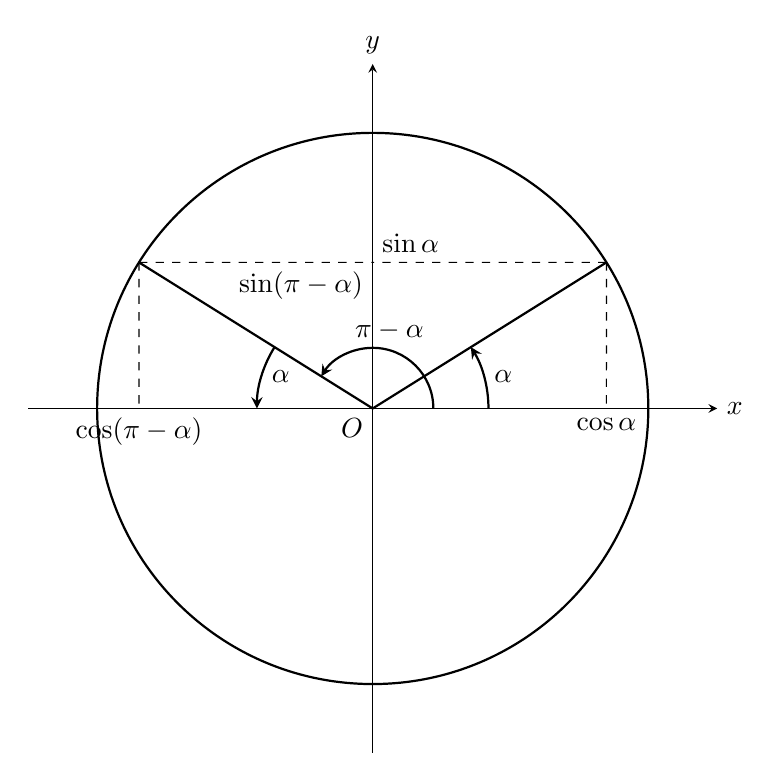
\begin{tikzpicture}[scale=3.5, >=stealth]

	\def\R{1}
	\def\ang{32} % angle in degrees

	\coordinate (O) at (0,0);

	\coordinate (P) at ({cos(\ang)},{sin(\ang)});
	\coordinate (Q) at ({cos(180-\ang)},{sin(180-\ang)});
	\coordinate (R) at (-1,0);

	\node[below left] at ($(O)$) {$O$};

	% axes
	\draw[->] (-1.25,0) -- (1.25,0) node[right] {$x$};
	\draw[->] (0,-1.25) -- (0,1.25) node[above] {$y$};

	% unit circle
	\draw[thick] (O) circle (\R);

	% radius to point P
	\draw[thick] (O) -- (P);

	% radius to point Q
	\draw[thick] (O) -- (Q);

	% projections
	\draw[dashed] (P) -- ({cos(\ang)},0)
	node[below] {$\cos\alpha$};
	\draw[dashed] (P) -- (0,{sin(\ang)})
	node[above right] {$\sin\alpha$};

	\draw[dashed] (Q) -- ({cos(180-\ang)},0)
	node[below] {$\cos(\pi-\alpha)$};
	\draw[dashed] (Q) -- (0,{sin(180-\ang)})
	node[below left] {$\sin(\pi-\alpha)$};

	% angle arc
	\draw[->, thick]
	(0.42,0) arc (0:\ang:0.42)
	node[midway, right] {$\alpha$};

	% angle arc
	\draw[->, thick]
	(0.22,0) arc (0:180-\ang:0.22)
	node[midway, above] {$\pi-\alpha$};

	% angle arc
	\draw[<-, thick]
	(-0.42,0) arc (0:-\ang:-0.42)
	node[midway, right] {$\alpha$};

\end{tikzpicture}
\end{document}
